\documentclass[11pt]{article}
\usepackage[T1]{fontenc}
\usepackage[utf8]{inputenc}
\usepackage{lmodern}
\usepackage[margin=1in]{geometry}
\usepackage{amsmath,amssymb,amsthm,mathtools}
\usepackage{booktabs,longtable,array,enumitem,microtype,graphicx,xcolor}
\usepackage{fancyhdr,listings}
\usepackage[colorlinks=true,linkcolor=blue!45!black,citecolor=blue!45!black,urlcolor=blue!55!black,breaklinks=true]{hyperref}
\hypersetup{pdftitle={Affine Geometry and Fast Cauchy Transforms for Subexponential SAT},pdfauthor={Research prepared for Vladimir Reshetnikov}}
\newtheorem{theorem}{Theorem}[section]
\newtheorem{lemma}[theorem]{Lemma}
\newtheorem{proposition}[theorem]{Proposition}
\newtheorem{corollary}[theorem]{Corollary}
\theoremstyle{definition}\newtheorem{definition}[theorem]{Definition}
\theoremstyle{remark}\newtheorem{remark}[theorem]{Remark}
\newcommand{\poly}{\operatorname{poly}}
\newcommand{\pc}{\operatorname{popcount}}
\newcommand{\ceil}[1]{\left\lceil#1\right\rceil}
\newcommand{\floor}[1]{\left\lfloor#1\right\rfloor}
\newcommand{\K}{\mathcal K}
\newcommand{\norm}[1]{\left\lVert#1\right\rVert}
\newcommand{\pin}{\texttt{a7ae5ab55f9627f5af7bf77443b3c34ef8ef1be4}}
\newcommand{\ap}{\texttt{1a6eee293b9e00cb432eef6018a21f523623a9af}}
\newcommand{\baseurl}{https://github.com/VladimirReshetnikov/ProveIt/blob/a7ae5ab55f9627f5af7bf77443b3c34ef8ef1be4/Computability/SubexponentialSAT/Research/}
\setlength{\headheight}{14pt}
\setlength{\emergencystretch}{3em}
\setlist{topsep=5pt,itemsep=3pt}
\pagestyle{fancy}\fancyhf{}
\fancyhead[L]{\small Affine geometry and fast Cauchy transforms}
\fancyhead[R]{\small Research report}
\fancyfoot[C]{\thepage}
\lstset{basicstyle=\ttfamily\small,columns=fullflexible,breaklines=true,frame=single,framerule=.3pt}
\newcommand{\Ctime}{30.413348726348439\ldots}
\newcommand{\Cspace}{29.466030256594790\ldots}

\title{Affine Geometry and Fast Cauchy Transforms\\for Subexponential SAT\\[6pt]
\large A smaller certified contraction exponent, exact local transforms,\\and a comparison with the newly published Anthropic formalization}
\author{Research prepared for Vladimir Reshetnikov}
\date{October 26, 2026 (Pacific date)}
\begin{document}
\maketitle
\begin{abstract}
We review ProveIt's four rounds of subexponential-SAT refinements at
commit \texttt{a7ae5ab55f}, including all nine newly placed round-4 packets, and the Anthropic
formal-math revision supplied during this review. A new finite geometric
construction lowers the strongest explicit generic cached-contraction bound
from time coefficient $30.891018920366\ldots$ to $\Ctime$, and from space
coefficient $30.753912832055\ldots$ to $\Cspace$, on the normalized scale
$s/\sqrt{\lceil\log_2s\rceil}$. Four parallel classes of the affine plane
$\mathbb F_3^2$ and a thirteen-plan cyclic construction provide exact
correlation certificates. A fully paid recursion includes every child entry.
Separately, we give precision-safe fast applications of the normalized
Cauchy feature matrix. At odd interpolation nodes the application reduces
to one convolution; exact tests and matched small benchmarks accompany it.
These are new improvements relative to the inspected corpus. They do not
establish a smaller logarithmic order for unrestricted SAT. We explain why
a direct combination with Anthropic's clique algorithm does not by itself
remove that obstacle, and isolate a conditional graded-algebra route and
an obstruction to its most immediate construction.
\end{abstract}
\setcounter{tocdepth}{1}
\tableofcontents
\newpage
\section{Results and their scope}

The strongest new result is a strictly smaller certified exponential
upper bound for the same generic normalized contraction problem used by
the most recent packets. Set $\lambda=\ceil{\log_2s}$ and
$E(s)=s/\sqrt\lambda$. The exact coefficients are
\begin{align}
 C_T&=\frac\pi{\ln2}
 \left(\frac49\sqrt{\frac{2000000}{15773}}
             +\frac{160\sqrt{14}}{351}\right)=\Ctime,\label{eq:headline-time}\\
 C_S&=\frac\pi{\ln2}\sqrt{\frac{2000000}{47319}}=\Cspace.
 \label{eq:headline-space}
\end{align}
Under the interface of Section~\ref{sec:interface}, time is
$(s+\mathcal L)^{O(1)}2^{(C_T+o(1))E(s)}$ and space is
$(s+\mathcal L)^{O(1)}2^{(C_S+o(1))E(s)}$.
Eventual coefficients $30.414$ and $29.467$ are certified by exact rational
interval calculations. The square-root ceiling changes no leading constant
relative to the $s/\sqrt{\log_2s}$ scale used by some other packets.

\begin{center}
\begin{tabular}{p{7.5cm}rr}
\toprule
Generic normalized certificate & Time & Space\\\midrule
Best reviewed polynomial-space branch \cite{flags}&46.184846&polynomial\\
Best reviewed cached branch \cite{treecert}&30.891019&30.753913\\
New menus, earlier three-stage schedule&30.512927&29.487537\\
New menus, final four-stage schedule&\textbf{30.413349}&\textbf{29.466030}\\
\bottomrule
\end{tabular}
\end{center}

The new cached time coefficient is about $1.5463\%$ smaller and its space
coefficient about $4.1877\%$ smaller than the strongest displayed comparable
generic cached result. These percentages compare coefficients, not observed
run times. If $U_{\rm old}$ and $U_{\rm new}$ denote the explicit
upper-bound expressions, then
\[
 \log_2\frac{U_{\rm old}}{U_{\rm new}}
 =\left(0.477670194017653\ldots+o(1)\right)E(s).
\]
This is a meaningful asymptotic improvement of the upper-bound function;
it is not a lower bound on the time consumed by the older algorithm.

\paragraph{The new idea.}
The earlier best cached proof selected among three contraction trees and
enumerated all tuples of their operation supports. We replace that small
unstructured menu with a finite geometric menu and a pairwise correlation
certificate. The nine-group construction uses the four parallel classes of
$\mathbb F_3^2$; the thirteen-group construction uses cyclic shifts of one
explicit seed. The certificate controls every feasible allocation of mode
weights, including table construction. It pays for every actual recursive
child-factor evaluation. This is a corpus-relative contribution; averaging,
finite geometry, and fast matrix multiplication are classical tools.

\paragraph{A second, local asymptotic improvement.}
The normalized Cauchy matrix need not be materialized to compute its source
linear forms. We give guarded product-tree algorithms for matrix-vector
application and its transpose. At odd interpolation nodes, the features
have a diagonal--Toeplitz--diagonal representation after known powers of
two are cleared. All source forms then require one convolution. In the
scalar ring this admits bit cost
$\widetilde O(N(p+N))$, hence $\widetilde O(Np)$ for $p\ge N$, including
the precision guards. The reviewed streamed application uses quadratic
feature work. The prototype's one-convolution specialization is faster on
all five reported fixtures; the general product-tree prototype is slower
at those sizes, and those regressions are retained.

\paragraph{The requested larger breakthrough remains open.}
The global SAT order remains
\[
 \poly_k(n,m)2^{O_k(n\log\log n/\sqrt{\log n})}
\]
in the unrestricted fixed-width case and
$2^{O_{k,D}(n/\sqrt{\log n})}\poly(n,m)$ at fixed clause density.
No $n/\log n$ algorithm is proved here. The complete deliverable separates
the new proved finite lemmas, imported analytic and arithmetic ingredients,
tested implementation, and genuinely conditional ideas. No end-to-end SAT
solver or new Lean formalization is claimed.

The coefficients above are per normalized Boolean wire $s$. They cannot be
inserted unchanged in an exponent written in SAT variables $n$. The
existing density-sensitive and low-degree branches remain in the available
portfolio; they have different premises. Nor can a numerical coefficient
be claimed to dominate an unspecified constant in the new Anthropic
big-$O$ bound. These distinctions are necessary to make the comparison
mathematically meaningful.

\section{Recent commits, the full comparison set, and the supplied PR}
\label{sec:review}

\subsection{Pinned review and incoming arrivals}
The review is frozen at ProveIt commit \pin. It was committed at
20:15:51 Pacific on October 26, 2026. The relevant progression is:
\begin{center}\small
\begin{tabular}{p{3.5cm}p{10.5cm}}
\toprule
Commit & Relevant action\\\midrule
\texttt{2b925d8800} & Places the seven first-round packets and primary manuscripts.\\
\texttt{3e09608991} & Vendors the OpenAI manuscript and its four LaTeX sources.\\
\texttt{6d3adc4506} & Places eight round-2 packets.\\
\texttt{450252e9d8} & Places five round-3 packets and restores two replay scripts.\\
\texttt{b9941a7396} & Commits the nine new incoming round-4 archives.\\
\texttt{a7ae5ab55f} & Places those nine packets under SubexponentialSAT.\\
\texttt{7de9d09fec} & Links the Anthropic formalization; no mathematical packet changes.\\
\bottomrule
\end{tabular}
\end{center}
At the review pin, \path{docs/incoming/} contains its README only. Its nine
recent SAT arrivals have already been relocated into the research tree.
They are included here; reviewing only the earlier fifteen or twenty packets
would give an obsolete benchmark. The review covered the 29 packet summaries
and status declarations, with detailed examination of the source interfaces
and leading proofs used in the new comparison. It did not independently
reprove every statement in all 29 packets.

The final branch check observed \texttt{7de9d09fecd17de776d712835ecb2011205c531d},
committed at 20:20:40 Pacific. We inspected its complete relevant diff:
it updates the README to link the Anthropic development and adds no
new proposal or complexity bound. The mathematical corpus remains pinned
at \pin; the documentation-only follow-up is recorded separately.

The accompanying source manifest records immutable source paths, Git blob IDs and
SHA-256 hashes. The checkout is unmodified. Historical archives and upstream
manuscripts are linked rather than duplicated in this deliverable.

\subsection{Inventory of the 29 refinement packets}
In the following table, PS denotes polynomial space. Cached coefficients
permit subexponential space. Unless qualified, numbers are generic
normalized-wire time coefficients reported by the corresponding packet,
with that packet's stated imported dependencies. This inventory summarizes
the indexed corpus \cite{corpus}; the new result uses the actual leading
interfaces, not just the printed decimal numbers.

\begin{longtable}{p{5.1cm}p{9.0cm}}
\toprule Packet & Relevant result or limitation\\\midrule
\endfirsthead
\toprule Packet & Relevant result or limitation\\\midrule
\endhead
\bottomrule\endfoot
\path{eth_contraction_improvements}&Sharper Hermite taper and streamed extraction; PS $648.441$.\\
\path{cauchy_mode_improvement}&Factorial modes; ratio $1/\sqrt3$ in the mode-enumeration constant.\\
\path{3sat_precision_refinement}&Precision $24MD/u\to6MD/u$; the stronger $n/\log n$-type rates need an unproved summation algorithm.\\
\path{sat_density_improvement}&Density-sensitive order envelope with $\min\{\log(2+m/n),\log\log n\}$.\\
\path{eth_density_refinement}&Independent intermediate-density improvement and constant refinements.\\
\path{3sat_refinement}&Scalar parity lift; second-contraction factorization remains missing.\\
\path{3sat_asymptotic_analysis}&Scoped taper, rank and degree barriers; conditional interfaces remain unconstructed.\\
\path{eth_asymmetric_packet_balancing}&PS $76.909$; asymmetric near-unit padding.\\
\path{3sat_round2_refinement}&PS $84.066$; independent source and actual-domain audit.\\
\path{eth_balanced_packing}&PS $94.748$; thin precision buffers and near-unit padding.\\
\path{eth_high_moment}&PS $94.748$; degree-sensitive extensions.\\
\path{eth_matching_refinement}&Third independent $94.748$ bound through matching-based packing.\\
\path{eth_packet_refinement}&PS $95.664$; improved pair loads.\\
\path{eth_recursive_refinement}&PS $133.207$; refined Cauchy residue classes.\\
\path{eth_joint_cauchy}&Full-block slope-four modes; PS $319.686$, cached $225.597$. Its mode identity is used by later improvements.\\
\path{sat_adaptive_contraction}&PS $55.709$; cached $36.750$; modular Cauchy kernels.\\
\path{sat_frontier_improvements}&PS $63.857$, cached $38.484$; variable arity and quadratic feature construction.\\
\path{subexponential_sat_frontier}&PS $63.852$, cached $37.930$; exact labeling and precision peeling.\\
\path{subexponential_sat_kernel_improvements}&PS composition $66.605$; Smith, streamed and projective coefficient kernels.\\
\path{subsat_contraction_tree}&Cached $35.355$; recursive table merging and a rational-matrix-to-ring bridge.\\
\path{sat_adaptive_bounds}&Best generic PS $46.184846$; complete binary flags. Low-degree cached $13.379649$ under stronger assumptions.\\
\path{sat_adaptive_tree_certificate}&Best generic cached $30.891019$ time and $30.753913$ space; adaptive three-plan support certificates.\\
\path{sat_adaptive_frontier}&PS $50.30469$; cached time/space $31.25240$.\\
\path{sat_adaptive_matrix_partition}&PS $50.21043$; cached $34.32528$.\\
\path{subexponential_sat_adaptive_four}&PS $50.39373$; cached $32.91581$, or $32.85635$ with the stated stronger matrix backend.\\
\path{subsat_rectangular}&PS $53.97753$; cached $33.99389$; precision and table barriers.\\
\path{eth_adaptive_exact_kernels}&PS $55.33162$, cached $35.07061$; sparse-support scoring and fused feature recurrences.\\
\path{3sat_round3_frontier}&PS $63.75736$; low-degree PS $23.66617$; centered extraction kernels.\\
\path{eth_adaptive_schedules}&PS $63.78117$, cached $37.59170$; an incremental matching-potential kernel.\\
\end{longtable}

All these packets retain the unrestricted SAT order. The strongest
established density-sensitive expression in the corpus is
\begin{equation}\label{eq:density}
 \poly_k(n,m)\,
 2^{O_k\left(\frac n{\sqrt{\log n}}
        \min\{\log(2+m/n),\log\log n\}\right)}.
\end{equation}
For example, $m=\Theta(n\log\log n)$ yields
$n\log\log\log n/\sqrt{\log n}$ in the exponent. This is an
intermediate-density improvement, not a smaller unrestricted order.
Conditional targets are not established algorithms that a new numerical
coefficient must beat.

\subsection{What the Anthropic revision changes}
During the review, the user supplied PR 31 of \path{anthropics/formal-math}
at exact revision
\begin{center}\ap.\end{center}
That revision publishes \path{eth/},
including the paper, the standalone theorem statements, the proof entry
point, the proof tree, and checking instructions \cite{anthropic}.
Accordingly, the earlier description of this formalization as unpublished
is stale; ProveIt's final documentation-only commit also corrects it.
This is a change in source availability and inspectability, not a
new smaller exponent stated in the PR.

\path{MainResults.lean} states the existence of one finite-alphabet
Mathlib multi-stack Turing machine and one constant $C$, both quantified
before $k,n$ and the formula. Under $k\ge1$, $n\ge4$, $m\ge2$, no repeated
clause-list, and occurrence of every declared variable, its bound is
\[
 2^{C\min\{km/\sqrt{\log_2m},\,
             k^2n\log_2\log_2n/\sqrt{\log_2n}\}}.
\]
\path{Solution.lean} supplies unconditional theorem terms through
\path{CountedRoute.mainTheoremHolds}; the ETH statement follows through
the named renaming and decision wrappers. There are 1,052 Lean files in
the inspected revision. The two actual \texttt{sorry} terms found by the
source scan are the intentionally unproved comparison statements in
\path{Challenge.lean}; the proof entry point does not import that file.
The comparator configuration lists the standard axioms
\texttt{propext}, \texttt{Classical.choice}, and \texttt{Quot.sound}, and
requests \texttt{nanoda} checking.

These are source-inspection findings. We did not install the pinned Lean
toolchain, rebuild the 1,052-file development, or replay its kernel checks.
A text scan for \texttt{sorry} is not a substitute for such a build.
The PDF at the supplied revision is not byte-identical to ProveIt's earlier
\path{claude-2o-n-3sat/eth.pdf}; both hashes are recorded. We therefore
read the supplied paper directly instead of assuming the earlier PDF was
the same document.

The newly available source is relevant to the mathematical search. Its
clique algorithm admits arbitrary integer-valued high-degree node tables, and its sharp
decomposition uses a graded operator algebra with partition-number growth.
Section~\ref{sec:order-research} examines both the possible composition with the
Cauchy method and the growth-rate suggestion in its Appendix H.

\section{The common contraction interface}
\label{sec:interface}

\subsection{What is inherited and what is changed}
The root problem is the exact contraction of a bipartite Boolean tensor
network with at most $s$ wires, at most polynomially many vertices, and
maximum degree at most $\ceil{s^{9/10}}$. Its description length is
$\mathcal L$. Initial entries lie in
\[
 (\mathbb Z/2^{P_0}\mathbb Z)[V]/(V^\ell),\qquad 1\le P_0,\ell\le s,
\]
and uniform entry evaluation has time
$(s+\mathcal L)^{O(1)}2^{O(s^{9/10})}$ and polynomial space, with fixed
constants. The desired contraction is
\[
 Z=\sum_{x\in\{0,1\}^{E}}\prod_v T_v(x|_{\delta(v)}).
\]
We use the exact deformation, integral evaluations, tapered Hermite recovery,
and immutable creation-precision convention of the source and refinements
\cite{openai,asymmetric,joint,flags,treecert}. A retained tensor is evaluated
at its creation precision and its canonical coordinates are reused; the
canonical-lift map is never assumed to preserve multiplication or addition.
Our new global result changes the summation of an already exact finite
expression. Its algebraic validity does not depend on experimental timings.

The auxiliary ring is a finite free extension
\[
 \mathcal A_p=(\mathbb Z/2^p\mathbb Z)[U,V]/(f(U),V^\ell),
\]
where $f$ is monic of degree $O(\log s)$ with irreducible reduction modulo
two. All precisions and coordinate lengths remain polynomial in $s$.
Arithmetic in this ring therefore introduces fixed polynomial factors.

\subsection{Packing, modes, and exact list cardinalities}
At depth $d$ let $u_d$ be the taper range, let
$B=\ceil{6\log_2\lambda}$ for $\lambda=\ceil{\log_2s}$, and put
\[
 a_d=\sum_{j\le d}(u_j+B),\qquad L_d=2^{a_d},\qquad Q_d=r_d^{a_d}.
\]
For a retained interpolation node of valuation $i<u_d$, set
$D=L_d/2^i$. The imported sharp precision estimate is
\begin{equation}\label{eq:precision}
 p_t\le(6+o(1))MD/u_d.
\end{equation}
Nearly lossless asymmetric packing makes each group child have at most
$(2/r_d+o(1))M$ wires. Sufficient packing conditions, suppressing fixed
polylogarithmic slack, are
\begin{equation}\label{eq:packing}
 Q_dR/M=o(1),\quad Q_d^2C(\log s)^2/M=o(1),\quad
 L_dQ_d^2/M=o(1).
\end{equation}
At the root both degree bounds are $\ceil{s^{9/10}}$; subsequently one may
take retained-side degree $R\le\ceil{s^{9/10}}$ and fresh-side degree
$C\le 2L_{d-1}$. The concrete schedule below verifies all these conditions.

Full-orientation Cauchy modes have weights at least
$1+4q-2\pc(q)$ after lowering the common positive valuation offset. There
are at most $(2/r^2+o(1))M/D$ modes of each index on a prescribed directed
pair. Enumerate exact pair-weight arrays $b=(b_{gh})$ whose sum is less
than $p_t$. The alphabet $r$ is fixed, so the number of these arrays is
polynomial in $s$. Let $\mathcal I_{gh}$ be the finite list of mode tuples
of the specified exact weight. Arrays with an empty list contribute zero.
For every remaining array the expression is exactly
\begin{equation}\label{eq:groupidentity}
 \sum_{(\xi_{gh})\in\prod_{g\ne h}\mathcal I_{gh}}
    \prod_{g=1}^r Z_g((\xi_e)_{e\ni g}).
\end{equation}
Each $Z_g$ entry is a genuine child-network contraction, not a free oracle.

List sizes and rank/unrank operations follow from
\[
 N(j,b)=N(j-1,b)+N(j,b-w_j),\quad N(0,0)=1,
\]
with zero for negative budgets and for $N(0,b)$ with $b>0$. Budgets,
table dimensions, and bit lengths of counts are polynomial in $s$.
This makes the selectors used later explicit exact algorithms.

\subsection{The entropy estimate}
Write $h_{gh}=\log_2|\mathcal I_{gh}|$ and
\[
 \kappa=\frac{\pi\sqrt2}{\ln2},\qquad
 \K(M,u)=\kappa M/\sqrt u.
\]
The common weighted estimate is the following.

\begin{lemma}[Imported weighted pair entropy]\label{lem:entropy}
For every fixed nonnegative directed weight vector $z$,
\[
 \sum_{g\ne h}z_{gh}h_{gh}
 \le\left(\frac{\norm z_2}{r}+o(1)\right)\K(M,u).
\]
The error is uniform over the active nodes and any fixed finite collection
of weight vectors used below.
\end{lemma}
\begin{proof}
The argument is included to expose the constant being used. The generating
product for one mode family satisfies
\[
 \sum_{q\ge0}-\ln(1-e^{-\theta(1+4q-2\pc(q))})
   =\frac{\pi^2}{24\theta}+O(\log^2(2/\theta)).
\]
The weight-counting function is $x/4+O(\log(x+2))$; partial summation and
$\int_0^\infty-\ln(1-e^{-x})\,dx=\pi^2/6$ give this estimate.
For positive $z_e$ use the parameter $\theta/z_e$ and multiply the
logarithm of its bound by $z_e$. Summing yields leading terms
\[
 \theta p_t+\frac{\pi^2}{24\theta}
              \frac{(2+o(1))M}{r^2D}\sum_ez_e^2.
\]
Optimizing and using \eqref{eq:precision} gives the claim after division
by $\ln2$. The saddle has scale $\sqrt u/D$; the additive guard makes the
error $o(M/\sqrt u)$ uniformly. Zero coordinates are omitted. A fixed
finite collection permits taking the largest of its error constants.
\end{proof}

\subsection{Cached matrix operations over the actual ring}
For disjoint blocks $A,B$ and their complement $O$, let $H_1,H_2,H_3$
be the logarithms of the products of index sizes on $A$--$O$,
$A$--$B$, and $B$--$O$. The block-table merge is rectangular matrix
multiplication. Square blocking with any rational-field matrix exponent
strictly below $12/5$ gives exponent
\begin{equation}\label{eq:matrix}
 \mu(H)=H_1+H_2+H_3-\frac35\min(H_1,H_2,H_3)
 =\max_j\left(\frac25H_j+\sum_{k\ne j}H_k\right).
\end{equation}
The cited matrix result is stronger than the inequality needed here
\cite{matrix}. We retain the exact coordinate/CRT bridge already proved
in the cached-tree packet \cite{cachedtree}. A brief explanation is useful:
expand the coefficient ring into polynomially many coordinates, lift
coordinates to integers, and perform the integer coordinate matrix products
modulo enough nonexceptional odd primes. A fixed rational bilinear matrix
algorithm has only finitely many denominator primes to exclude. CRT
reconstructs integer products before applying the ring's structure constants
and reducing modulo $2^p$. Reconstruction lengths are polynomial in $s$
and the logarithms of matrix dimensions. No nonunit of $\mathcal A_p$ is
inverted in this argument.

The matrix bound dominates every input and output table size because
$\mu(H)\ge H_j+H_k$ for distinct $j,k$. Sequential rectangular blocking
and the fixed bilinear algorithm use a polynomial factor times that
storage. Reshaping, indexing, and sorting also cost only a polynomial
factor in record and index lengths. The verification code does not
implement the theoretical fast matrix backend; that backend is an
explicit imported dependency.

\section{Affine and cyclic menus with pairwise correlation certificates}
\label{sec:menus}

\subsection{Operation supports and exact selection}
For an unordered pair $e=\{g,h\}$ put $g_e=h_{gh}+h_{hg}$.
A plan partitions the ordered group labels into three nonempty blocks.
Within each block, recursively split its ordered list after
$\floor{k/2}$ elements and merge the two boundary tables. Finally contract
the three block tables. This gives $r-3$ binary merges and one final
triangle, hence $r-2$ operations.

Multiplying each of the three linear forms in \eqref{eq:matrix} by five
gives a support mask $v\in\{0,2,5\}^{\binom r2}$. Its value is zero
inside a class of the operation's tripartition, two on the discounted
class pair, and five on the other two class pairs. Let $\mathcal V_j$
contain all $3(r-2)$ masks of plan $j$. After singleton caching, plan $j$
has local operation exponent
\[
 F_j(g)=\frac15\max_{v\in\mathcal V_j}v\cdot g.
\]
All matrix operations, not only the last triangle, are included.

\begin{theorem}[Pairwise correlation certificate]\label{thm:gram}
For $q$ fixed plans on $r$ groups, let $D_{ij}$ be any explicit upper bound
on $v\cdot w$ for $v\in\mathcal V_i,w\in\mathcal V_j$, and put
$S=\sum_{i,j}D_{ij}$. Selecting the least-cost plan gives local time and
storage at most
\[
 \poly(s)2^{(b_r+o(1))\K(M,u)},\qquad
 b_r^2=\frac{2S}{25q^2r^2}.
\]
The selector is exact and polynomial time in the original size parameter.
\end{theorem}
\begin{proof}
For the given nonnegative $g$, choose a maximizing $v_i$ from each menu.
Then
\[
 \min_i F_i(g)\le\frac1{5q}\left(\sum_i v_i\right)\cdot g,
 \qquad
 \left\|\sum_i v_i\right\|_2^2
       =\sum_{i,j}v_i\cdot v_j\le S.
\]
Give both directed orientations of edge $e$ the weight
$(\sum_i v_i)_e/(5q)$. Its squared norm is at most $2S/(25q^2)$.
Lemma~\ref{lem:entropy} proves the time estimate. The possible choices of
supports form a fixed finite set, so the error remains uniform although
the selected plan depends on the input. No minimax equality is assumed.

For selection, compute the exact positive integers
\[
 P_i=\max_{v\in\mathcal V_i}
       \prod_{\{g,h\}}
       (|\mathcal I_{gh}|\,|\mathcal I_{hg}|)^{v_{\{g,h\}}}
\]
and choose the smallest. Comparing them is equivalent to comparing
$F_i(g)$; no approximate logarithm is needed. Their bit lengths are
polynomial and $q,r$ are fixed. Finally every table is an input or output
of a selected operation, whose exponent dominates its size by
\eqref{eq:matrix}. A fixed number of tables introduces only a constant
factor. The time to evaluate the singleton entries is charged separately.
\end{proof}

The earlier support-tuple method has an exponential dependence on the
number of plans, even though this remains a constant asymptotically. The
new certificate requires $q^2$ pair comparisons. It bounds the simultaneous
sum of supports rather than asserting that all pairwise maxima can occur
at once. Such an assertion would be unnecessary and generally false.

\subsection{Four parallel classes on nine points}
Label the groups by $x\mapsto(x\bmod3,\floor{x/3})\in\mathbb F_3^2$.
For each of the four functionals
\[
 (a,b)\in\{(1,0),(0,1),(1,1),(1,2)\},
\]
use its three
level sets as the final blocks. Within each level set use increasing
integer order. These four plans are
\[
\begin{split}
 &(0,3,6)\mid(1,4,7)\mid(2,5,8),\\
 &(0,1,2)\mid(3,4,5)\mid(6,7,8),\\
 &(0,5,7)\mid(1,3,8)\mid(2,4,6),\\
 &(0,4,8)\mid(1,5,6)\mid(2,3,7).
\end{split}
\]
\begin{figure}[ht]
\centering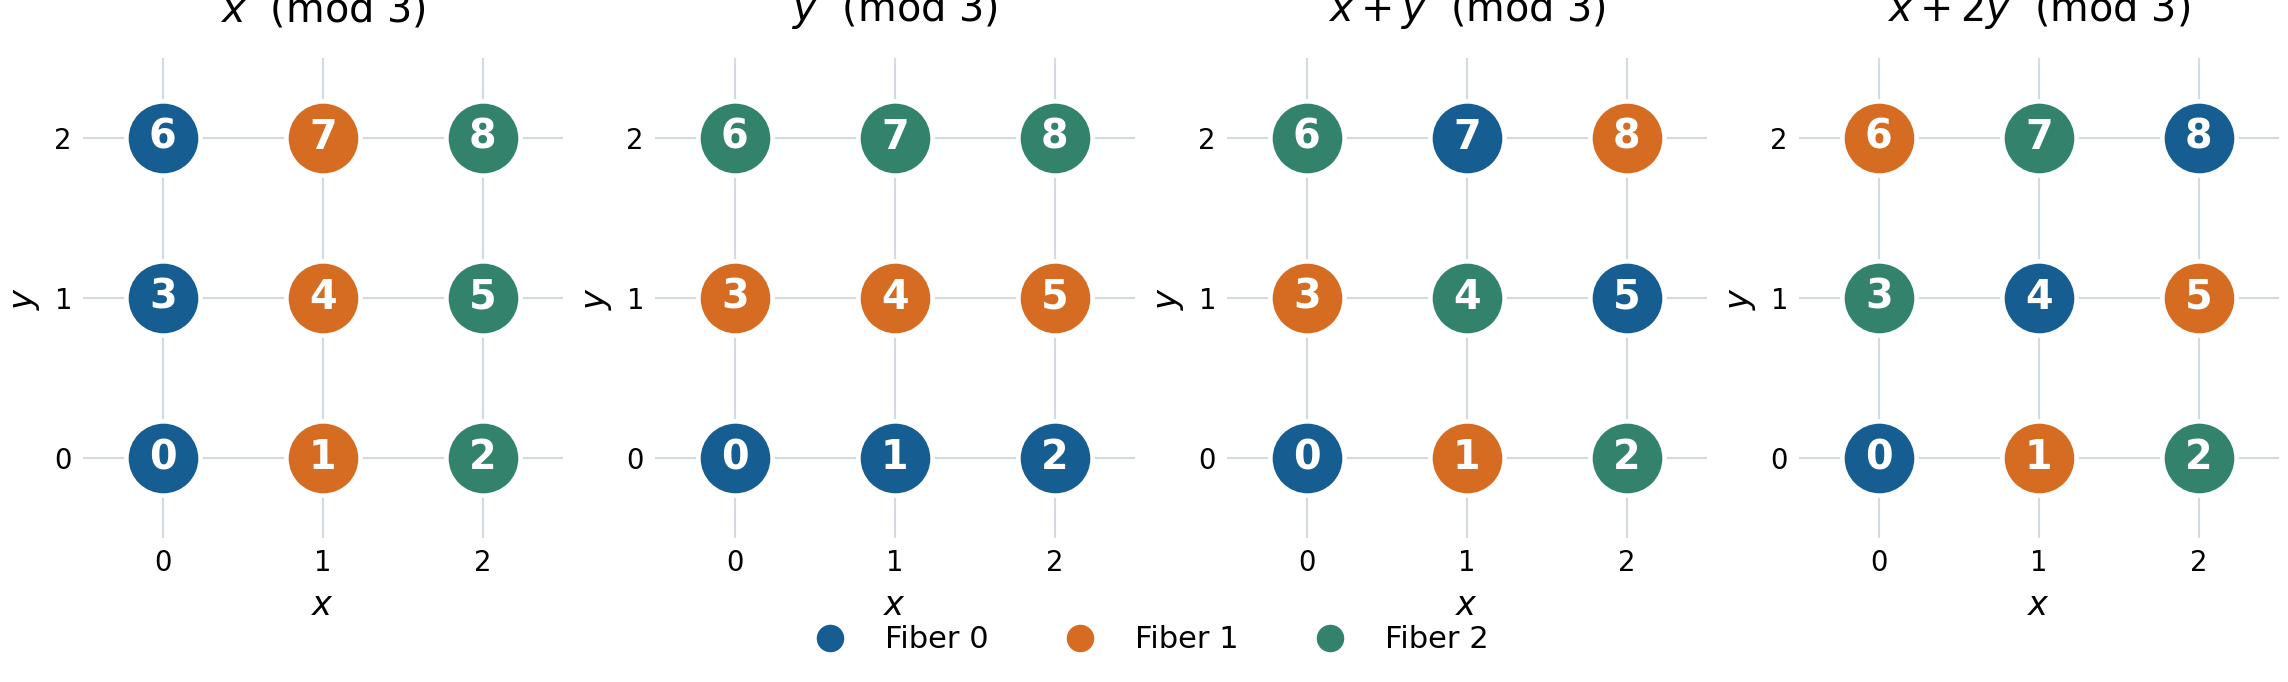
\includegraphics[width=\textwidth]{figures/affine_classes.png}
\caption{The four parallel classes of $\mathbb F_3^2$. In each panel,
colors denote the three fibers of the indicated linear functional, with
arithmetic modulo three. Labels are the group numbers. Each fiber is one
final block; straight Euclidean lines are not required to display the
modular wraparound.}
\end{figure}

Each plan has 21 masks. Exact pairwise maxima are
\[
 D_{ii}=486,\qquad D_{ij}=288\quad(i\ne j).
\]
Thus $S=4\cdot486+12\cdot288=5400$ and
\begin{equation}\label{eq:b9}
 b_9^2=\frac13.
\end{equation}
This can be checked by 7,056 mask-pair dot products, not by sampling
entropy vectors. The independent implementation represents each support
as $v=5\mathbf1_C-3\mathbf1_D$ and uses
\begin{equation}\label{eq:intersection}
 v\cdot w=25|C\cap C'|-15(|D\cap C'|+|C\cap D'|)+9|D\cap D'|.
\end{equation}

There is also a geometric explanation for the largest off-diagonal value.
Two distinct directions have a one-point intersection between every pair
of their lines. For the final triangles, the two crossing edge sets have
intersection size 18; either discounted set meets the other crossing set
in 6 edges, and the discounted sets meet in 2. Equation~\eqref{eq:intersection}
then gives $25\cdot18-15(6+6)+9\cdot2=288$.
For completeness, the exact off-diagonal bounds by operation type are
\[
\begin{array}{c|rrr}
 & (1,1,7)&(1,2,6)&(3,3,3)\\\hline
 (1,1,7)&204&208&215\\
 (1,2,6)&208&240&260\\
 (3,3,3)&215&260&288
\end{array}
\]
where the triples specify the class sizes of an operation. The finite
enumeration covers all of them, including the ordering-dependent internal
merges.

\subsection{Thirteen cyclic plans}
Take the ordered seed
\[
 (11,2,8,9,7)\mid(10,1,0,5)\mid(6,4,3,12)
\]
and add $d$ modulo 13 to every label for $0\le d<13$. The within-block
orders remain the shifted orders; sorting them would define different
plans. There are 33 masks per plan. The maximum-dot matrix is circulant,
with first row
\[
 (1064,647,651,713,647,709,651,651,709,647,713,651,647).
\]
Its row sum is 9,100. Hence $S=118,300$ and
\begin{equation}\label{eq:b13}
 b_{13}^2=\frac{56}{169}.
\end{equation}
The checker exhausts 184,041 mask-pair dot products. The seed was found by
an exploratory search. Its validity depends only on this explicit seed
and the complete integer checks; no optimality or exhaustive seed search
is claimed.

For the final six-group tail use
$(0,1)\mid(2,3)\mid(4,5)$. Its final triangle has maximum squared mask
norm 216 and each internal merge at most 204, giving
$b_6^2=2\cdot216/(25\cdot6^2)=12/25$.

\subsection{Why the gain is not merely schedule slack}
The earlier best three-plan nine-group certificate has
$b_{9,\rm old}^2=6608/18225$ \cite{treecert}. In the same packing model,
the root taper fraction satisfies $\eta_0<1/(20\log_2 9)$. Even pushing
that certificate to its boundary leaves root coefficient at least its
infimum
\[
 \kappa b_{9,\rm old}\sqrt{20\log_2 9}
 =30.731244617454\ldots,
\]
which is larger than our complete time coefficient. Thus our improvement
cannot be reproduced solely by reclaiming the rational slack of that
particular old root certificate. This is a statement about the displayed
certificate model; it is not an algorithmic lower bound or a global
optimization over all methods in the corpus.

% Replacement global-schedule section. Retain affine/cyclic menu lemma above.
\section{A strict four-stage schedule: coefficient below 30.414}
The new finite menus permit a better fully charged schedule than simply
replacing the menus of the prior $9\to13\to7$ certificate.
Use the nine-group affine menu, the thirteen-group cyclic menu, the same
nine-group affine menu once more, and then a fixed six-group tail.
The tail plan is $(0,1)\mid(2,3)\mid(4,5)$. Its final triangle has mask
squared norm $4\cdot4+8\cdot25=216$, and its other merges have maximum
squared norm $204$. Thus its local coefficient satisfies $b_6^2=12/25$.

Let $\lambda=\lceil\log_2s\rceil$ and define
\[
\begin{array}{c|c|c}
 d&r_d&\eta_d\\\hline
0&9&15773/10^6\\
1&13&9/800\\
2&9&4477/10^6\\
d\ge3&6&(923/250000)(12/25)^{d-3}.
\end{array}
\]
Set $u_d=\lfloor\eta_d\lambda\rfloor$,
$B=\lceil6\log_2\lambda\rceil$, $a_{-1}=0$, $a_d=\sum_{j\le d}(u_j+B)$,
and stop at $M\le H=\lceil s/\lambda^{3/4}\rceil$.
Use relative padding slack $\lambda^{-3}$ and retain the imported frozen
creation-precision entry semantics. Finite small exceptions are handled
by direct contraction, after checking all applicability gates.

The prefix sums are
\[
 \eta_0+\eta_1=27023/10^6,\qquad
 \eta_0+\eta_1+\eta_2=63/2000.
\]
The tail sums to $71/10000$, so total taper capacity is $193/5000$.
The following exact integer inequalities certify all required logarithms:
\[
 9^{20000}<2^{63399},\quad
 13^{2000}<2^{7401},\quad
 9^{100}<2^{317},\quad
 6^{200}<2^{517}.
\]
For the symmetric root gate $Q_0^2s^{9/10}$, then the retained-side gates
$Q_ds^{9/10}$, they give the respective fixed gaps below exponent one
\[
 \frac{7573}{10^{10}},\qquad
 \frac{2777}{2\cdot10^9},\qquad
 \frac{29}{200000},\qquad
 \frac{219}{10^6}.
\]
All gaps are strict. In particular the thirteen-group logarithm is bounded
by $7401/2000$, rather than the weaker $3701/1000$ which would not suffice
for this schedule. The fresh-side degree term and packet-rounding term are
bounded by leading exponent
\[
 \frac{193}{5000}\left(2\frac{7401}{2000}+1\right)
 =\frac{1621393}{5000000}<1.
\]
New degrees have exponent at most $193/5000+o(1)<9/10$.

To close the depth argument without assuming padding in advance, consider
hypothetical active tail depths at most $\frac34\log_2\lambda+O(1)$.
The least retained taper is
\[
 \lambda^{\varepsilon+o(1)},\qquad
 \varepsilon=1-\frac34\log_2(25/12)>0,
\]
where $(25/12)^3<16$ is an exact certificate. The cumulative buffers are
$O((\log\lambda)^2)$, and $s/M<\lambda^{3/4}$. Hence the fixed positive
packing gaps absorb all guards and polylogarithmic losses uniformly in
this hypothetical depth range. Padding is nearly lossless and the true
tail child ratio is $1/3+o(1)<1/2$, closing the depth bootstrap.
The product of relative padding errors over $O(\log\lambda)$ levels is
$1+o(1)$, and the floors are uniformly relative $o(1)$.

Every retained valuation satisfies $D\ge2^{a_{d-1}+B+1}$. The inherited
creation precision $O(s\lambda^2 2^{a_{d-1}})$ divided by $MD/u_d$ is at
most $O(\lambda^{15/4}2^{-B})=o(1)$. Thus the same sharp local precision,
weighted entropy, and entry-evaluation interfaces apply uniformly.
The wire counts satisfy
\[
 M_0\le s,\quad M_1\le(1+o(1))\frac{2s}{9},\quad
 M_2\le(1+o(1))\frac{4s}{117},\quad
 M_d\le(1+o(1))\frac{8s}{1053}\left(\frac13\right)^{d-3}
 \quad(d\ge3).
\]

Write $K_d:=\K(M_d,u_d)$ and $\alpha_r=\sqrt{2(r-1)}/r$.
The local paid recurrence is
\[
 T_d\le\operatorname{poly}(s)
 \left[2^{(\alpha_{r_d}+o(1))K_d}T_{d+1}
       +2^{(b_{r_d}+o(1))K_d}\right],
\]
with $b_9=1/\sqrt3$, $b_{13}=\sqrt{56}/13$, $b_6=\sqrt{12}/5$.
The singleton cache must be evaluated by the actual child contraction;
its cost is the first term, not a unit-cost oracle.
On the scale $s/\sqrt\lambda$, define
\[
\begin{split}
 K_0^*&=\kappa\sqrt{10^6/15773},\qquad
 K_1^*=\kappa\frac29\sqrt{800/9},\\
 K_2^*&=\kappa\frac4{117}\sqrt{10^6/4477},\qquad
 K_3^*=\kappa\frac8{1053}\sqrt{250000/923}.
\end{split}
\]
The tail ratio is $\gamma=(1/3)/\sqrt{12/25}=5/(6\sqrt3)$.
Since $\alpha_6/(1-\gamma)>b_6$, unrolling the recurrence bounds every
branch by the maximum of
\[
\begin{aligned}
 C_0&=b_9K_0^*=29.466030256594790\ldots,\\
 C_1&=\alpha_9K_0^*+b_{13}K_1^*
      =30.413348726348439\ldots,\\
 C_2&=\alpha_9K_0^*+\alpha_{13}K_1^*+b_9K_2^*
      =29.634547541824756\ldots,\\
 C_\infty&=\alpha_9K_0^*+\alpha_{13}K_1^*+\alpha_9K_2^*
              +\frac{\alpha_6}{1-\gamma}K_3^*
      =30.013332173441237\ldots.
\end{aligned}
\]
All displayed comparisons are enclosed by rational intervals in the
checker, rather than inferred from rounded floating-point values.

The resulting exact time and space coefficients are
\[
\boxed{\displaystyle
 C_T=\frac\pi{\ln2}
 \left(\frac49\sqrt{\frac{2000000}{15773}}
            +\frac{160\sqrt{14}}{351}\right)
 =30.413348726348439\ldots}
\]
and
\[
\boxed{\displaystyle
 C_S=\frac\pi{\ln2}\sqrt{\frac{2000000}{47319}}
 =29.466030256594790\ldots.}
\]
The local storage coefficients after the root are respectively
$7.73038806\ldots$, $1.89085996\ldots$, and
$0.55525285\ldots$; they are smaller than $C_S$.
Ancestor tables add in size, so their exponents are maximized, not added.
Direct leaves cost $2^{O(s/\lambda^{3/4})}$, original entry evaluation
costs $2^{O(s^{9/10})}$ times a polynomial, and new entry routines cost
$\exp(s^{193/5000+o(1)})$; all are lower order.
The product of fixed polynomial overheads over $O(\log\lambda)$ levels
adds $O(\lambda\log\lambda)=o(s/\sqrt\lambda)$ to the time exponent.

Thus, under the same explicit imported contraction interface, the improved
algorithm uses deterministic time
\[
 (s+\mathcal L)^{O(1)}2^{(C_T+o(1))s/\sqrt\lambda}
\]
and space with the same form and coefficient $C_S$.
The safe eventual coefficients $30.414$ and $29.467$ are certified.
This strictly improves the inspected generic cached certificates
$30.891018920366\ldots$ time and $30.753912832055\ldots$ space.
It remains a coefficient improvement on the same logarithmic scale,
not a proof of a stronger unrestricted SAT exponent order or an observed
end-to-end runtime improvement.

\section{Fast, precision-safe Cauchy feature application}
\label{sec:transforms}

\subsection{A different local interface}
The global theorem above reduces the cost of summing mode indices. This
section improves a different step: evaluating all source linear forms at a
given port assignment. Earlier packets give quadratic feature-table
construction or quadratic streamed application \cite{joint,kernels,cachedtree}.
The output of a full $N\times N$ table already has quadratic size. A
matrix-vector product has only linear input and output size and need not
materialize that table. We exploit this distinction.

Fast polynomial products, multipoint evaluation, transposed algorithms,
and Toeplitz convolution are classical \cite{mca}. The contribution here
is their exact realization for the corpus's normalized two-adic features,
including the extra precision required by the normalization. We found no
such implementation or argument in the inspected packet text. This is a
corpus-relative finding, not a claim of priority for fast structured linear
algebra in general.

Let $L=2^a$, $N=L/2$, $R=2^i$ with $0\le i<a$, and define the
increasing orientation slots
\[
 s_j=(j\bmod R)+2R\floor{j/R}\qquad(0\le j<N).
\]
Let $T$ be a specified element of valuation $i$ in the unramified
coefficient ring, available at the increased precision required below.
The source has $T=t+2^{a+1}\zeta$ with a fixed canonical description, so
such evaluation is available. For $\epsilon\in\{1,-1\}$ put
$x_j=\epsilon s_j$, $z_b=\epsilon s_b$ and
\[
 E_b=2\floor{b/R}-\pc(\floor{b/R}).
\]
The normalized features of \cite{joint} are
\begin{equation}\label{eq:features}
 F_{jb}=2^{-E_b}\frac{T}{T+x_j-z_b}
             \prod_{h<b}\frac{x_j-z_h}{T+x_j-z_h}.
\end{equation}
They are integral and vanish for $j<b$. Positive sign gives the target
features; negative sign gives the source features, commonly denoted $G$.
Thus the source forms are precisely $G^{\mathsf T}v$ for the vector of
real column bits. Omitted ports may be omitted from the sum or zero-filled.
We allow the first $1\le B\le N$ modes and any specified set $J$ of real ports.
Vector entries may belong to the finite free nilpotent extension as well.
Canonical lifts of vector entries can be chosen freely: integrality of
$F$ makes the output modulo $2^p$ independent of those choices. This does
not assert that canonical lifting is a ring homomorphism.

\subsection{The denominator valuations}
Let
\[
 D_B(X)=\prod_{h<B}(T+X-z_h),\qquad H=E_{B-1}.
\]
The sequence $E_b$ is nondecreasing. For $j\in J$, the known valuation of
the denominator is
\begin{equation}\label{eq:denvaluation}
 \kappa_j=v_2(D_B(x_j))
   =\sum_{d=1}^{i}\#\{h<B:h\equiv j\pmod{2^d}\}.
\end{equation}
Indeed the slot difference has valuation either below $i$ or strictly
above $i$; both slots have bit $i$ equal to zero. Since $v_2(T)=i$,
the summand denominator has valuation $\min(i,v_2(j-h))$, with $i$ for
$j=h$. Counting divisibility levels proves \eqref{eq:denvaluation}.
For $\kappa=\max_{j\in J}\kappa_j$, with zero for an empty set,
\[
 \kappa\le B(1-1/R)+i,\qquad H\le2(B-1)/R.
\]
In particular,
\begin{equation}\label{eq:guards}
 H+\kappa\le2B+i,\qquad H+2\kappa\le2B+2i.
\end{equation}
The implementation uses the exact valuations, not merely these upper bounds.

\subsection{Synthesis by a rational Newton product tree}
For a consecutive interval $I=[l,r)$ define
\[
 A_I(X)=\prod_{h\in I}(X-z_h),\quad
 B_I(X)=\prod_{h\in I}(T+X-z_h),
\]
and, with $w_b=c_b2^{H-E_b}T$,
\[
 C_I(X)=\sum_{b\in I}w_b
    \prod_{l\le h<b}(X-z_h)
    \prod_{b<h<r}(T+X-z_h).
\]
For consecutive halves $I=I_1\cup I_2$ the identity
\begin{equation}\label{eq:producttree}
 C_I=C_{I_1}B_{I_2}+A_{I_1}C_{I_2}
\end{equation}
is division free. At the root,
\[
 (Fc)_j=\frac{C_{[0,B)}(x_j)}{2^H D_B(x_j)}.
\]
Build the product tree and evaluate the numerator and denominator at all
$x_j$ modulo $2^{p+H+\kappa}$. Monic product/remainder trees need only
division by monic polynomials, so no nonunit leading coefficient is
inverted. By integrality of $F$, the numerator at $x_j$ is divisible
by $2^{H+\kappa_j}$. Divide that power of two exactly, invert the unit
part of the denominator, and reduce modulo $2^p$. The guard leaves at
least $p$ correct bits. All unit inverses can be obtained by one batch
inverse and linear multiplication work.

\subsection{The transpose requires a separate guard}
It would be invalid simply to transpose an algorithm that contains
divisions by powers of two. We instead derive a division-free linear
map and justify its final divisions directly.

Put $P=p+H+\kappa$. First build and evaluate $D_B$ at precision
$P_{\rm high}=p+H+2\kappa$. Its normalized units
$u_j=D_B(x_j)/2^{\kappa_j}$ are then known modulo $2^P$.
Batch-invert them and set
\[
 w_j=2^{\kappa-\kappa_j}u_j^{-1}v_j\pmod{2^P}.
\]
For $N_b(X)=\prod_{0\le h<b}(X-z_h)\prod_{b<h<B}(T+X-z_h)$, compute
$q_b=\sum_jN_b(x_j)w_j$ as follows. First obtain the first $B$ moments
\[
 m_k=\sum_jw_jx_j^k
\]
from the first $B$ coefficients of $\sum_jw_j/(1-x_jZ)$. A balanced
numerator/denominator construction and power-series inversion do this.
The series denominator has constant coefficient one. Newton inversion
$g\leftarrow g(2-fg)$ works in this ring; it does not require that two
be invertible.

Next transpose the division-free recurrence \eqref{eq:producttree}.
If $d$ is the parent coefficient functional, its child functionals are
\[
 d_1[k]=\sum_t B_{I_2}[t]d[k+t],\qquad
 d_2[k]=\sum_t A_{I_1}[t]d[k+t].
\]
Each is a polynomial correlation. At the leaves the resulting values
are the $q_b$. Finally,
\begin{equation}\label{eq:transposefinal}
 (F^{\mathsf T}v)_b=\frac{Tq_b}{2^{\kappa+E_b}}\pmod{2^p}.
\end{equation}
The numerator is divisible by the displayed power because $F$ is
integral. Since $E_b\le H$, the core precision $P$ leaves at least $p$
bits. The higher precision for denominator preparation is essential:
normalizing a denominator first consumes $\kappa_j$ bits before its
unit inverse is used at precision $P$.

\begin{theorem}[Fast guarded feature application]\label{thm:transform}
Let $m=B+|J|$. Both synthesis and the transposed source-form map can be
computed without a dense feature table in
\[
 O\bigl(\mathsf M_{\mathcal A}(m,p+O(B+i))\log(m+2)\bigr)
\]
arithmetic cost, plus linear unit arithmetic and a batch inverse, where
$\mathsf M_{\mathcal A}$ is polynomial-multiplication cost over the actual
coefficient algebra. A stored product tree uses $O(m\log(m+2))$
coefficient storage. The required precisions are respectively
$p+H+\kappa$ and $p+H+2\kappa$ for synthesis and transpose preparation.
\end{theorem}
\begin{proof}
The preceding identities prove correctness. At each balanced-tree level
the total polynomial degree is $O(m)$; standard superlinear
multiplication-cost bounds sum to the displayed complexity. Monic
remainders, constant-one series inversion, and correlations have the
same multiplication-based bounds. The storage bound counts the
coefficients across tree levels. Equations~\eqref{eq:guards} give the
precision assertion.
\end{proof}

\subsection{Odd interpolation nodes need only one convolution}
When $i=0$ the formula simplifies substantially: $s_j=2j$ and $T$ is a
unit. Let
\[
 f_j=v_2(j!)=j-\pc(j),\quad o_j=j!/2^{f_j},\quad
 D_j=\prod_{h=0}^j(T+2\epsilon h),\quad D_{-1}=1,
\]
and put $u_j=o_j/D_j$, $v_j=D_{j-1}/o_j$. All these denominators are
units. Direct cancellation in \eqref{eq:features} gives
\begin{equation}\label{eq:toeplitz}
 F_{jb}=\epsilon^bT\,
  2^{f_j-f_b-f_{j-b}}u_jv_{j-b}\qquad(j\ge b).
\end{equation}
The exponent equals $v_2\binom jb\ge0$. To verify the identity, the
numerator product in \eqref{eq:features} is
$(2\epsilon)^b j!/(j-b)!$, the denominator product is
$D_j/D_{j-b-1}$, and $E_b=b+f_b$.

\begin{theorem}[One-convolution source forms]\label{thm:oneconv}
For all $N$ modes and ports at $i=0$, either $Fc$ or $F^{\mathsf T}v$
is computable with one polynomial convolution, $O(N)$ preparation,
and one batch inverse at precision $p+2f_{N-1}$.
\end{theorem}
\begin{proof}
Set $K=f_{N-1}$ and $V_t=2^{K-f_t}v_t$ at that precision.
For synthesis convolve $V$ with
$c'_b=c_b\epsilon^bT2^{K-f_b}$. Multiply coefficient $j$ by $u_j$ and
divide by $2^{2K-f_j}$; equation~\eqref{eq:toeplitz} gives $(Fc)_j$.
For the transpose correlate $V$ with $a_j=v^{\rm input}_j2^{f_j}u_j$.
At index $b$, multiply by $\epsilon^bT$ and divide by $2^{K+f_b}$.
Again \eqref{eq:toeplitz} gives exactly the desired answer. One reversed
polynomial product yields all correlations. Each division is exact and
consumes at most $2K$ bits. The odd parts $o_j$ and products $D_j$ are
prepared by recurrence and batch inversion in linear work.
\end{proof}

In the scalar ring, quasi-linear integer multiplication with Kronecker
substitution gives $\widetilde O(N(p+N))$ bit operations, including
the guard. It is therefore $\widetilde O(Np)$ when $p\ge N$. The
coefficient algebra's rank must be included for extension rings, or one
can leave the cost as $\mathsf M_{\mathcal A}$. The executable supplied
here implements the scalar ring with CPython integers. It does not
implement an optimal FFT backend or an optimized extension-ring version.

Taking $p=p_t$ at the active-node scale $p\asymp MD/u$ and $N=RD/2$ gives
$p/N\asymp 2M/(Ru)$. Under the fixed schedule of this report,
$R\le2^u=s^{\eta_d+o(1)}$, while active $M>s/\lambda^{3/4}$.
Thus the extra $O(N)$ bits are lower order than the active precision.
This argument must be rechecked for a different schedule; it is not a
license to omit guards from a general complexity claim.

Finally, these transforms evaluate linear source forms. The subsequent
nonlinear mode monomials and the paid child contractions still have to be
summed. The transforms alone therefore leave the global exponent scale
unchanged. Their benefit is a provable local asymptotic improvement and,
for the odd-node specialization, a measured improvement on the supplied
small kernel fixtures.

\section{What the new source changes about the order question}
\label{sec:order-research}

The new cached coefficients improve a certified exponential constant.
They leave the worst-case scale
$n\log\log n/\sqrt{\log n}$ unchanged.  The user-supplied Anthropic
development introduces a different algebraic mechanism, and therefore
deserves more than a comparison of its headline bound.  This section
examines a possible composition, makes one of the source's suggested
extensions precise, and proves a restricted obstruction to a natural
implementation of that extension.

\subsection{A direct composition spends the apparent extra saving}

The earlier precision packet gives an exact rank encoding of the
structured mode sum \cite{precision}.  If the first deformation uses
$r$ groups, its existing collision-packing certificate allows a retained
level range of order
\[
 u\asymp\frac{\log M}{\log r}.
\]
Its compressed mode-index graph consequently has a certified bit budget
on the scale
\begin{equation}
 B\asymp\frac{M}{\sqrt u}
       \asymp\frac{M\sqrt{\log r}}{\sqrt{\log M}}.
 \label{eq:composition-budget}
\end{equation}
These are the scales of that proof's envelopes, not lower bounds on the
actual entropy of every instance.

At fixed or polylogarithmic $r$, a group tensor can have degree comparable
to $B/r$, so the original bounded-degree contraction theorem cannot
simply be invoked again at size $B$.  This missing interface is already
identified in the earlier reports \cite{precision,barriers}.
Anthropic's complete-graph algorithm does permit arbitrary integer-valued node tensors
with charged entry access \cite[Theorem A]{anthropic}.  It is therefore a
more appropriate possible backend, after balancing and representation
costs have been supplied.

However, the inspected backend has an exponent rate of order
$e(r)\asymp1/\sqrt{\log r}$ along its certified schedule.  Even the
optimistic calculation that leaves out balancing and entry-evaluation
overheads gives
\begin{equation}
 e(r)B\asymp
 \frac1{\sqrt{\log r}}
 \frac{M\sqrt{\log r}}{\sqrt{\log M}}
 =\frac{M}{\sqrt{\log M}}.
 \label{eq:composition-cancellation}
\end{equation}
For fixed $r$ the backend changes a constant.  Increasing $r$ spends
the corresponding saving in the first-stage retained-level budget.
Allowing $r$ to grow would also require uniform accounting for the
exact-weight arrays and the newly expensive group entries.  Equation
\eqref{eq:composition-cancellation} is thus a diagnosis of this proposed
composition, not a completed composition theorem or an algorithmic lower
bound.  The new source resolves an important admissibility mismatch but
does not automatically supply the missing $M/\log M$ summation method.

\subsection{A cost-complete form of the source's growth suggestion}

Appendix B of the Anthropic paper builds crossing decompositions from
operators on the graded space
$V=\mathbb Q[t_1,t_2,\ldots]$, with $\operatorname{weight}(t_j)=j$.
Here $\dim V_E=p(E)$ is the ordinary partition number.  Its two operator
orders pass through spaces of weights at most $2h+s$ and $2h-s$.
The asymptotic relation $\log_2p(E)=A\sqrt E+O(\log(E+2))$ gives the
rank-sum parameter $\rho=1/\sqrt2$ and the logarithmic exponent
$\log_2(1/\rho)=1/2$ \cite[Appendices A and B]{anthropic}.

The source itself observes in Appendix H that growth like $E^\beta$
would instead give $\rho=2^{\beta-1}$.  The following proposition
formalizes that suggestion with the resource hypotheses needed for an
algorithm.  The growth-to-rate idea belongs to the source.  No algebra
meeting the stronger hypotheses below is constructed in this report.

\begin{proposition}[Conditional graded-growth transfer]
\label{prop:graded-growth}
Fix a rational $0<\beta<1$.  Suppose an effectively presented graded rational
operator system $V=\bigoplus_{E\ge0}V_E$ has fixed bases, finite,
nondecreasing dimensions $d_E\ge1$, and
\begin{equation}
 \log_2d_E=A E^\beta+O(\log(E+2)),\qquad A>0.
 \label{eq:graded-growth}
\end{equation}
For each bit length $b$, let $h$ be the least integer with $d_h\ge2^b$
and label $2^b$ distinct basis states of $V_h$ by $x\in\{0,1\}^b$.
Assume the following additional properties, uniformly in $b$.
\begin{enumerate}
\item A nondegenerate dual pairing and an exact operator identity give
operators $Q_s(x,v)$ on $V_h$, for $|s|\le2h$, and a positive integer
$D_h$, such that
\[
 \sum_{s=-2h}^{2h}Q_s(x,v)=D_h[x=v]\operatorname{Id}_{V_h}.
\]
\item Each $Q_s(x,v)$ has two exact factorizations, respectively as a
sum of $h^{O(1)}$ products $B_{v,s,j}A_{x,s,j}$ and as a sum of
$h^{O(1)}$ products $\widetilde A_{x,s,j}\widetilde B_{v,s,j}$.
The intermediate spaces in the first factorization have weights at
most $2h+s$, and those in the second at most $2h-s$.
All factorization entries are integral, after any specified common
denominator clearing.  This exact two-order identity is a hypothesis;
a dimension estimate alone does not imply it.
\item There are uniform algorithms computing $h$, labels, index lists,
$D_h$, piece values and factorization entries in $2^{O(b)}$ bit
operations.  The number of pieces is $b^{O(1)}$, and all integers have
$b^{O(1)}$ bits.  In particular the hypotheses include the basis and
rank-decoding costs and effective exact locality, wherever locality is
used to prove the preceding identities.
\end{enumerate}
Then the system supplies pieces in Anthropic's Definition 7 with
$\rho=2^{\beta-1}$.  Relative to its Theorem A and dense reduction, this
gives, for fixed width $k$,
\[
 \poly(n,m)2^{O_k(n\log\log n/(\log n)^{1-\beta})}
\]
time at arbitrary density and
$\poly(n,m)2^{O_{k,D}(n/(\log n)^{1-\beta})}$ when $m\le Dn$.
No polynomial-space conclusion is part of this implication.
\end{proposition}

\begin{proof}
For a piece define
$A_s(x,y,u,v)=\langle e_u^*,Q_s(x,v)e_y\rangle$, where $e_u^*$ is
the dual basis vector.
The first identity gives
$\sum_s A_s=D_h[x=v][y=u]$.
The first factorization separates $(x,y)$ from $(u,v)$, and the
second separates $(x,u)$ from $(y,v)$.  By monotonicity of $d_E$,
their respective numbers of rank terms are at most
$h^{O(1)}d_{2h+s}$ and $h^{O(1)}d_{2h-s}$.

The matching upper and lower estimates in \eqref{eq:graded-growth},
together with minimality of $h$, give
\[
 h=\Theta(b^{1/\beta}),\qquad
 A h^\beta\le b+O(\log(b+2)).
\]
Indeed $d_{h-1}<2^b$ supplies the latter inequality up to
$A(h^\beta-(h-1)^\beta)=O(1)$.  Rounding the logarithms of the
rank term counts to bits and using concavity of $x^\beta$ gives
\begin{align*}
 c_s^{\rm row}+c_s^{\rm col}
 &\le A\bigl((2h+s)^\beta+(2h-s)^\beta\bigr)+O(\log h)\\
 &\le 2A(2h)^\beta+O(\log h)\\
 &\le 2^{\beta+1}b+O(\log(b+2)).
\end{align*}
Thus Definition 7 holds with $4\rho=2^{\beta+1}$; its other
conditions are precisely the effective hypotheses above.  Finitely
many small values of $b$ can be absorbed by enlarging its fixed
constant.  Theorem A has logarithmic exponent
$\log_2(1/\rho)=1-\beta$.  For fixed rational $\beta$, the rational
rate approximations required by that theorem are computable by integer
power comparisons, so its stated consequences apply.
\end{proof}

For example, $\beta=1/3$ would replace the square-root denominator by
$(\log n)^{2/3}$.  This is a sufficient-condition calculation, not an
achieved improvement.  Even $\log d_E=\Theta(E^\beta)$ is insufficient
to identify the displayed $\rho$: unrelated constants in the upper
and lower estimates would remain in the rank bound.

\subsection{Why deleting oscillator modes does not realize it}

A natural candidate retains only square-weight generators,
$\mathbb Q[t_1,t_4,t_9,\ldots]$.  Its attraction is the smaller
partition growth.  Its immediate defect is that the current's positive
commutator series has the form
\begin{equation}
 C(z)=\sum_{j\ge1}j^2z^{j^2},
 \label{eq:square-current}
\end{equation}
up to a monomial shift or nonzero coefficient normalization.
It cannot satisfy the polynomial-clearing locality used in Appendix B.
The obstruction extends beyond this one choice.

\begin{lemma}[Rational series cannot have unbounded support gaps]
\label{lem:rational-gaps}
Let $C(z)=\sum_{n\ge0}c_nz^n$ over a field be rational and not a
polynomial.  After a finite prefix, its nonzero coefficient support has
bounded gaps.
\end{lemma}
\begin{proof}
Write $Q(z)C(z)=P(z)$ with $Q(0)=q_0\ne0$ and $d=\deg Q$.
For $n>\deg P$ the coefficients satisfy
\[
 q_0c_n+q_1c_{n-1}+\cdots+q_dc_{n-d}=0.
\]
If $d$ consecutive coefficients in this tail were zero, induction
would force every later coefficient to vanish.  This would make $C$
a polynomial.  The case $d=0$ already makes $C$ a polynomial and is
excluded.  Therefore sufficiently late gaps have length less than $d$.
\end{proof}

The series \eqref{eq:square-current} has arbitrarily long zero runs
between consecutive squares and infinitely many nonzero terms, so it is
not rational.  In particular, no nonzero polynomial $Q$ makes $QC$ a
polynomial.  In the independent-current construction, clearing the
two-variable commutator by a fixed power of $(\omega_1-\omega_2)$
would, on taking its positive expansion and setting
$z=\omega_2/\omega_1$, imply just such rationality.  More explicitly,
up to a monomial shift the two-sided scalar distribution is
$C(z)-C(z^{-1})$.  Multiplying its negative part by $(1-z)^N$ can
produce positive exponents only below $N$.  Thus annihilation of the
distribution forces all sufficiently high coefficients of
$(1-z)^NC(z)$ to vanish.  The square-weight
replacement therefore lacks the exact identity on which the claimed
rank bounds would depend.

\begin{proposition}[A growth obstruction for independent oscillators]
\label{prop:oscillator-growth}
Let $S\subseteq\mathbb Z_{>0}$ be infinite and be the nonzero
coefficient support, apart from finitely many indices, of a rational
nonpolynomial current series.  Give the polynomial space
\[
 V=\mathbb Q[t_n:n\in S]
\]
the grading $\operatorname{weight}(t_n)=n$.  There is $c>0$ such that,
for all sufficiently large $E$,
\begin{equation}
 \sum_{j=0}^E\dim V_j\ge2^{c\sqrt E}.
 \label{eq:cumulative-growth}
\end{equation}
Consequently this model cannot satisfy a uniform exact-degree upper
bound $\dim V_E\le\exp(O(E^\beta+\log(E+2)))$ with $\beta<1/2$.
\end{proposition}
\begin{proof}
By Lemma~\ref{lem:rational-gaps}, a fixed integer $d$ bounds the gaps
in $S$ after a finite prefix.  For sufficiently large $B$, at least
$B/(2d)$ members of $S$ lie in $[1,B]$.  Independently choosing
exponent zero or one on these generators produces at least
$2^{B/(2d)}$ distinct monomials, every one of weight at most
$B|S\cap[1,B]|\le B^2$.  Take $B=\lfloor\sqrt E\rfloor$.
This proves the cumulative, rather than pointwise, lower bound
\eqref{eq:cumulative-growth}.  On the other hand, the proposed
exact-degree upper bound would imply
\[
 \sum_{j=0}^E\dim V_j
 \le (E+1)\exp\bigl(O(E^\beta+\log(E+2))\bigr),
\]
contradicting \eqref{eq:cumulative-growth} when $\beta<1/2$.
\end{proof}

The independence in this proposition is not removed by taking a
quotient that preserves a nondegenerate Heisenberg vacuum
representation.  Suppose a nonzero vacuum $v_0$ is annihilated by
positive operators $a_n$, the negative operators $a_{-n}$ raise weight
by $n$, operators of either sign commute among themselves, and
\[
 [a_n,a_{-m}]=\delta_{nm}\gamma_n\operatorname{Id},
 \qquad \gamma_n\ne0\quad(n\in S)
\]
over a characteristic-zero field.  In a relation among creation
monomials of the same weight, apply
$\prod_na_n^{\alpha_n}$ for any exponent tuple $\alpha$ appearing
there.  Every different same-weight tuple has some smaller coordinate
and is killed.  The matching tuple leaves
$\prod_n\alpha_n!\gamma_n^{\alpha_n}\,v_0\ne0$.
Hence its coefficient in the relation is zero, and all creation
monomials are independent.  Such a quotient retains the growth
obstruction.

These statements concern the specified independent-current or
Heisenberg-vacuum model.  They do not rule out different noncentral
operator algebras, other exact recovery identities, compressed tensor
representations, or faster SAT algorithms.  In particular, they are
not general lower bounds for vertex algebras or for SAT.  Their useful
conclusion is narrower: merely deleting oscillator modes, or imposing
relations while retaining the displayed Heisenberg premises, does not
implement the source's smaller-growth suggestion.

\subsection{Further research questions}

\begin{enumerate}
\item Can a noncentral graded operator algebra supply the pairing,
two-order identity and effective factorization of
Proposition~\ref{prop:graded-growth} with $\beta<1/2$?  A candidate
must escape the preceding Heisenberg premises while preserving exact
recovery and uniform bit costs.
\item Can a different exact recovery method use a nonrational current?
Truncating its commutator is insufficient unless the residual is proved
to vanish in the actual counting ring and the required precision is
fully charged.
\item Can the mode-rank and clique algorithms be composed with complete
balancing and entry-query accounting to improve a coefficient or the
memory tradeoff?  An order claim must additionally overcome
\eqref{eq:composition-cancellation}.
\item Which relations among the \emph{actual} group tensors permit
implicit summation without materializing their formal boundary tables?
Existing inventory barriers concern a representation; they do not
establish independence or noncancellation of the values in those tables
\cite{precision,barriers}.
\end{enumerate}

The first two questions seek a new algebraic ingredient.  The latter
two seek a representation that uses more than pair entropy.  None of
these required interfaces has been supplied here, so the proved
positive improvement remains the smaller cached contraction constant
and the exact kernel refinement established elsewhere in this report.

\section{Validation, reproducibility, and exact scope}
\label{sec:validation}

\subsection{What was checked}
The finite correlation certificates and the rational schedule are replayable
with the Python standard library. The main checker exhausts every support
pair: 7,056 dot products for the four affine plans and 184,041 for the
thirteen cyclic plans. The six-group tail is checked as well. Integer power
comparisons certify the logarithm bounds; rational interval arithmetic
certifies the displayed constants and strict dominance of the depth-one
time branch. In particular the final intervals are
\[
 \begin{aligned}
 C_T&\in[30.413348726348439,30.413348726348440],\\
 C_S&\in[29.466030256594790,29.466030256594791].
 \end{aligned}
\]
An independently written checker reconstructs the plans and their supports
using bit sets, recomputes the integer certificates and rational packing
gates, and directly unrolls 93 levels of the paid recurrence as a numerical
cross-check. It does not import the primary checker. The finite unrolling
is supplemental: the proof handles the infinite geometric tail exactly.

The regrouping test uses 12 deterministic fixtures with at most 12 active
binary directed indices. It compares literal enumeration of global
assignments with separately implemented singleton caches, balanced binary
merges and the final three-block sum over
$(\mathbb Z/64\mathbb Z)[V]/(V^2)$. All 72 plan contractions agree.
The fixtures cover both orientations, spanning paths, disconnected
components, isolated scalar factors and zero factors. The nine fixtures
without a zero factor all have nonzero outputs. The checker also counts
every singleton entry call, verifies the count $\sum_v2^{\deg(v)}$,
and checks that the exact fifth-power selector minimizes the independently
reconstructed operation costs. This is a finite check of regrouping and
resource accounting, not an implementation of fast matrix multiplication.

For the local transform, 246 cases compare with independently formed
exact rational feature matrices, covering 10,160 entries; 27 larger cases
compare with the quadratic valuation-aware recurrence; and 96 odd-node
cases check the convolution specialization. Both signs, truncated mode
lists, missing ports, precision one, and the adjoint identity are covered.
The denominator guard bounds are checked in these cases. These finite
tests support the implementation; the product-tree and precision arguments
in Section~\ref{sec:transforms} establish the general identities.

All deterministic checks pass in normal Python and in \texttt{python -O},
with identical parsed output. Validation uses explicit exceptions rather
than depending on assertions that optimization could remove. The archived
results include both modes and a summary of the comparison.

\subsection{Matched local measurements}
The following scalar transpose measurements include preparation,
denominator inversions, increased working precision, and output recovery.
Every measured output was checked against the quadratic implementation.
Each number is the median of three runs at $p=4N$ and odd interpolation
valuation. The code uses CPython integers and Kronecker substitution;
these are small local measurements, not an end-to-end SAT benchmark.
\begin{center}\small
\begin{tabular}{r r r r r}
\toprule
$N$ & Quadratic (s) & One convolution (s) & Ratio & General tree (s)\\
\midrule
32 & 0.000407 & 0.000174 & $2.34\times$ & 0.002486\\
64 & 0.001923 & 0.000853 & $2.25\times$ & 0.011521\\
128 & 0.013941 & 0.007689 & $1.81\times$ & 0.091038\\
256 & 0.168149 & 0.057822 & $2.91\times$ & 0.656261\\
512 & 1.706872 & 0.418585 & $4.08\times$ & 6.034264\\
\bottomrule
\end{tabular}
\end{center}
The general product-tree prototype is slower at all these sizes. Its
asymptotic coefficient-operation bound remains useful, but these data
do not establish a practical crossover. The observed speedup belongs to
the odd-node specialization. The reference environment was Python 3.12.14
on Linux 6.18.55, x86\_64, glibc 2.39. Raw samples and environment metadata
are included so the measurements are not mistaken for portable constants.

\subsection{Proof status and limitations}
The newly proved parts are the correlation-certificate inequality, the
explicit affine and cyclic menus, their integration into a fully charged
four-stage recurrence, the precision-safe rational transforms and odd-node
convolution, and the restricted sparse-current obstruction. The result
uses the established interfaces of the inspected manuscripts: exact
Hermite extraction, normalized mode factorization, balanced packing,
entry semantics, SAT reduction, and the rational matrix multiplication
backend. Those dependencies are stated in Section~\ref{sec:interface};
this report is not an independent verification of every upstream claim.

The new contraction algorithm permits subexponential space. It does not
improve the strongest polynomial-space bound, prove a smaller logarithmic
order for unrestricted SAT, provide a finite-size crossover threshold,
or contain an end-to-end SAT implementation. Neither this new proof nor
its upstream dependencies were formalized or replayed in Lean here. The
source review of the supplied Anthropic revision does not change that
statement. The conditional graded-algebra proposition requires a new
construction meeting all of its hypotheses.

\subsection{Reproducing the archive}
From the extracted directory, run:
\begin{lstlisting}
python3 code/check_manifest.py
python3 code/run_checks.py
python3 code/build_report.py
\end{lstlisting}
The first command checks the delivered file hashes. The second replays
the finite certificates, independent audits, regrouping and kernel tests
in both Python modes. It requires only Python 3.10 or later. PDF rebuilding
requires pdfLaTeX and the packages named in \path{report.tex}; the supplied
figure is already present. To regenerate it, install Matplotlib and run
\path{code/make_figures.py}. Optional fresh timings use
\texttt{python3 code/fast\_cauchy\_transform.py --benchmark}; they need not
match the archived timings. The exact proof obligations, imported
dependencies and unproved targets are also recorded in
\path{PROOF_STATUS.json}.

\begin{thebibliography}{99}
\bibitem{corpus}
Vladimir Reshetnikov, \emph{ProveIt: SubexponentialSAT}, project index and
29 refinement packets, commit \pin.
\href{https://github.com/VladimirReshetnikov/ProveIt/tree/a7ae5ab55f9627f5af7bf77443b3c34ef8ef1be4/Computability/SubexponentialSAT}{Immutable project tree}.
The companion provenance manifest supplies exact file hashes and paths.

\bibitem{placement}
ProveIt commit \texttt{a7ae5ab55f}, \emph{Place nine round-4
sub-exponential 3-SAT packets in SubexponentialSAT}, October 26, 2026 Pacific.
\href{https://github.com/VladimirReshetnikov/ProveIt/commit/a7ae5ab55f9627f5af7bf77443b3c34ef8ef1be4}{Commit and placement record}.

\bibitem{openai}
OpenAI, \emph{The Exponential Time Hypothesis is False}, October 25, 2026,
upstream commit \texttt{7ef5c0cc5ca4b0e072b7a050fca09ab24bc6fa3a}.
\href{https://github.com/openai/math/tree/7ef5c0cc5ca4b0e072b7a050fca09ab24bc6fa3a/preprints/The-Exponential-Time-Hypothesis-is-False-October-25-2026}{Pinned source directory}.
The unmodified ProveIt copy under \path{lib/openai-math/preprints/}
was read, especially \path{build/quantitative-contraction.tex} and
\path{build/quantitative-reduction.tex}.

\bibitem{anthropic}
Claude (Anthropic), \emph{A $2^{o(n)}$ Time Algorithm for 3-SAT}, paper
and Lean source in \path{anthropics/formal-math}, PR 31, revision \ap.
\href{https://github.com/anthropics/formal-math/tree/1a6eee293b9e00cb432eef6018a21f523623a9af/eth}{Pinned paper and formalization}.
Particularly Theorem A, Appendices B and H, \path{MainResults.lean},
\path{Solution.lean}, and \path{comparator.json}. Source inspected;
the Lean build and kernel replay were not run for this report.

\bibitem{precision}
\emph{Sharper precision for subexponential 3SAT}, October 26, 2026,
ProveIt \path{Research/3sat_precision_refinement/}.
\href{\baseurl 3sat_precision_refinement/report.tex}{Pinned report source}.
Used for sharp precision, the exact mode-rank encoding, and the explicitly
unproved stronger summation hypothesis.

\bibitem{barriers}
\emph{Asymptotic improvement analysis for the October 2026 3-SAT preprint},
ProveIt \path{Research/3sat_asymptotic_analysis/}.
\href{\baseurl 3sat_asymptotic_analysis/report/report.tex}{Pinned report source}.
Also \emph{Rectangular cached contraction},
\href{\baseurl subsat_rectangular/report.tex}{pinned source}, for scoped
precision and explicit-table barriers.

\bibitem{asymmetric}
\emph{Asymmetric packet balancing}, October 26, 2026,
ProveIt \path{Research/eth_asymmetric_packet_balancing/}.
\href{\baseurl eth_asymmetric_packet_balancing/report.tex}{Pinned report source}.
Used for the asymmetric packing gates and nearly lossless child sizes.

\bibitem{joint}
\emph{Joint Cauchy modes}, October 26, 2026,
ProveIt \path{Research/eth_joint_cauchy/}.
\href{\baseurl eth_joint_cauchy/report.tex}{Pinned report source}.
Used for full-orientation normalized rational features, their integrality,
and slope-four mode weights.

\bibitem{flags}
\emph{Adaptive bounds for subexponential SAT}, October 26, 2026,
ProveIt \path{Research/sat_adaptive_bounds/}.
\href{\baseurl sat_adaptive_bounds/report/report.tex}{Pinned report source}.
Includes the common weighted entropy interface and the best displayed
generic polynomial-space coefficient.

\bibitem{cachedtree}
\emph{Subexponential SAT contraction tree}, October 26, 2026,
ProveIt \path{Research/subsat_contraction_tree/}.
\href{\baseurl subsat_contraction_tree/report/cached_tree.tex}{Pinned cached-tree proof}.
Used for matrix table merging and the coordinate/CRT arithmetic bridge.

\bibitem{treecert}
\emph{Adaptive contraction trees with exact support certificates},
October 26, 2026,
ProveIt \path{Research/sat_adaptive_tree_certificate/}.
\href{\baseurl sat_adaptive_tree_certificate/report.tex}{Pinned report source}.
The leading comparable cached coefficient and the earlier strict
$9\to13\to7$ schedule come from this packet.

\bibitem{kernels}
\emph{Adaptive exact kernels}, October 27, 2026 archive date,
ProveIt \path{Research/eth_adaptive_exact_kernels/}.
\href{\baseurl eth_adaptive_exact_kernels/report.tex}{Pinned report source}.
Also \emph{SAT frontier improvements},
\href{\baseurl sat_frontier_improvements/report.tex}{pinned source}, and
the prefix theorem in \emph{Subexponential SAT contraction tree},
\href{\baseurl subsat_contraction_tree/report/prefix_theorem.tex}{pinned source}.
These are the reviewed quadratic feature-construction/application interfaces.

\bibitem{density}
\emph{Density-aware SAT improvement},
\href{\baseurl sat_density_improvement/density_aware_sat_improvement.tex}{pinned source},
and \emph{ETH density refinement},
\href{\baseurl eth_density_refinement/report.tex}{pinned source}.
Both appear in ProveIt at the review commit.

\bibitem{matrix}
J. Alman, R. Duan, V. Vassilevska Williams, Y. Xu, Z. Xu and R. Zhou,
\emph{More Asymmetry Yields Faster Matrix Multiplication},
arXiv:2404.16349v2, 2024.
\url{https://arxiv.org/abs/2404.16349v2}.
Only the strict rational-field inequality $\omega<12/5$ is needed here;
no current-record claim is made.

\bibitem{mca}
J. von zur Gathen and J. Gerhard, \emph{Modern Computer Algebra},
third edition, Cambridge University Press, 2013. Classical polynomial
product trees, monic division, fast series inversion and multipoint
evaluation underlie the transform construction.
\end{thebibliography}

\end{document}
